\section{The Reward Function}
\label{section:the-reward-function}

The main prerequisite of an environment that can be solved by the single-step method is that the agent has global information. There, the optimal representation of the reward function by the XCS is also the solution of the actual problem. For example in the 6-multiplexer problem the reward function already contains the table of the 6-multiplexer itself. 

In multi-step environments the environment only returns $1$ when the agent stands on the goal position and $0$ at all other positions. As there is only access to local information it is up to the individual agent to build up a reward function for all positions in order to be able to decide which direction is to be preferred at each step.

This is done by back propagating the reward of the environment to previous actions. During the back propagation the reward is discounted in order to favor shorter routes. When the goal position is reached the scenario is repeated a number of times. In order to find the optimal (shortest) route, i.\,e., the global reward function, the agent must be able to distinguish between all positions, i.\,e., the scenario must have the Markov property.

In the predator/prey scenario the nature of the reward function is not obvious. 
In such a dynamic environment with a continuous goal condition neither repetition is possible nor does that environment possess the Markov property. Other agents and the goal object may have moved and previously gathered information might be no longer valid.

Thus, global information and therefore a global reward function cannot be constructed and it is important to reward previous actions directly. In addition it is necessary to determine points in time when a reward is to be distributed because the simulation runs continuously.

In order to fulfil these requirements a new way of reward distribution for such a scenario has been developed. First the environment reward function is chosen by testing static strategies in the scenario (see Section~\ref{subsection:environment-reward-function}). Agents then record the resulting reward values and create \emph{events} when the values change or when there was no change for a specific amount of time (see Section~\ref{subsection:events}). After that previously executed actions are rewarded according to the type of and the time difference between the current and the last event (see Section~\ref{subsection:reward-distribution}).

\subsection{Environmental Reward Function}
\label{subsection:environment-reward-function}

A ``goal position'' in the context of a predator/prey scenario could be defined as ``be in observation range of the goal object'' which would be equal to the global goal. Another approach would be to make use of the increased abilities of the sensors of the agents instead of being restricted to a simple binary function as in some multi-step environments (``goal position reached'' and ``goal position not reached''). 

Because of the number of possible reward functions that include sensory information not all functions can be tested in a reasonable amount of time. Thus, this paper proposes another approach:

By looking at the global goal it is possible to examine reward functions by testing agents with static strategies instead of XCS. Although static strategies do not use a reward function, they still evaluate situations and corresponding actions either as ``good'' (``move in that direction'') or as ``bad'' (``don't move in that direction'').

Of a set of simple implementations the best results (except for some special cases like very large environments and a relatively small number of agents) delivered the following heuristic:

\begin{itemize}
	\item Cooperation (goal object not in sight) : Move in a random direction without other agents in sight.
	\item Egoism (goal object in sight): Move in the direction of the goal object.
\end{itemize}

Modelling this static strategy would require multiple states. As the original implementation uses a binary reward function the following approximation of the reward function $r_{b}(s_{a}, s_{g})$ with $s_{a}, s_{g}$ being indicators whether the goal object is in sight range ($s_{g} = true$) and whether any other agent is in sight range ($s_{a} = true$) is used:

$$
r_{b}(s_{a}, s_{g}) = \left\{ \begin{array}{rl}
  0 & s_{a} \wedge \overline{s_{g}} \\
  1 & \overline{s_{a}} \vee s_{g}
       \end{array} \right.
$$

As further adaptions to the reward is necessary the value this function returns will be called ``base reward'' and the function itself ``environmental reward function''. In the following section the actual reward for the rules of the XCS will be calculated. 

\subsection{Events}
\label{subsection:events}

Above we concluded that it is important to determine points in time when the reward is distributed. In the usual implementation of XCS~\cite{BW02} this happens whenever a positive reward is generated and the scenario is then restarted. Here, we analyze past base reward values and generate so called \emph{events} when either the \emph{base reward} value has changed or when there was no change for a certain period of time.

Assuming that the agent did something right when it gets into sight range of the goal object (or leaving the sight range of all other agents) such a situation change will be called a ``positive event'' while loosing the goal object or getting into sight range of other agents will be called a ``negative event''. Thus a positive event occurs whenever the base reward changes from $0$ to $1$, a negative event occurs whenever the base reward changes from $1$ to $0$ (see Figure~\ref{figure:positive-negative-events}).

\begin{figure*}[ht]
  \subfigure[Example of a series of base rewards that lead to positive and negative events.\label{figure:positive-negative-events}]{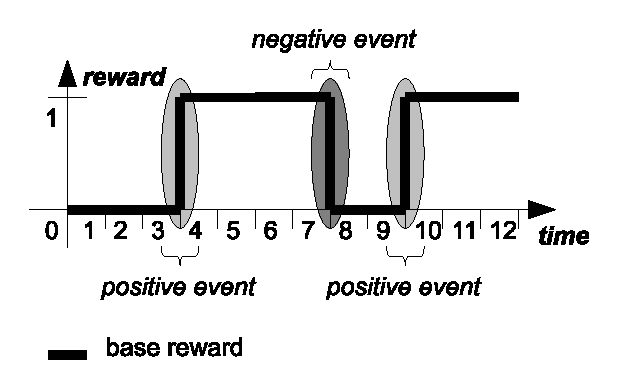
\includegraphics[width=0.33\textwidth]{positive_negative_events.eps}}\subfigure[Example of a series of base rewards that lead to neutral event (with \emph{maxStackSize} = 8).\label{figure:neutral-event}]{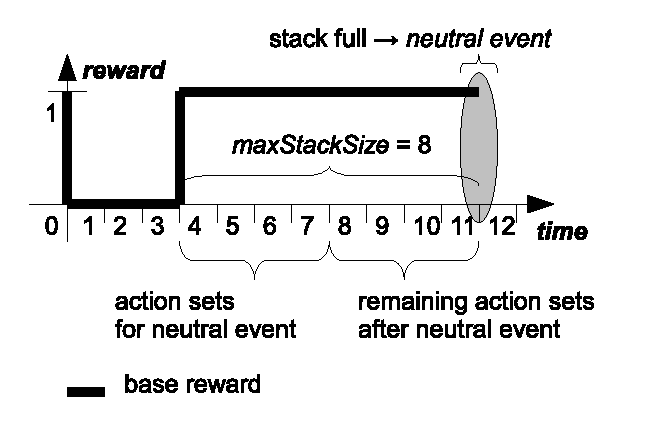
\includegraphics[width=0.33\textwidth]{neutral_event.eps}}\subfigure[Schematic presentation of the reward distribution to the action sets over time after several positive and negative events\label{figure:saved-rewards}]{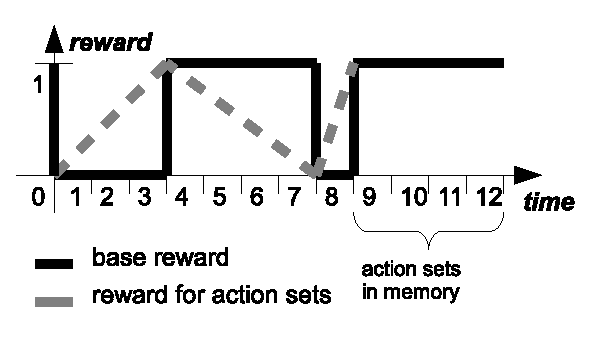
\includegraphics[width=0.33\textwidth]{saved_rewards.eps}}
\caption{\mathversion{bold}Calculation of the reward of individual action sets by analyzing the course of the base reward}\label{figure:experiment}
\end{figure*}

%\begin{figure}[ht]
%\centerline{	
%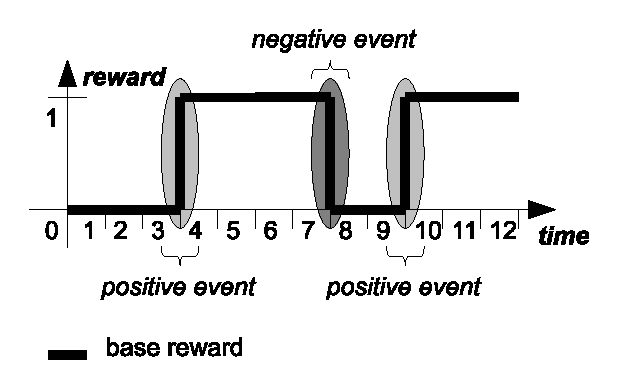
\includegraphics[scale=0.75]{positive_negative_events.eps}
%}
%\caption{Example of a series of base rewards that lead to positive and negative events.}
%\label{figure:positive-negative-events}
%\end{figure}

As there can be cases where an agent never encounters an event the number of steps is limited to \emph{maxStackSize} steps. If the step counter reaches that number then a ``neutral event'' occurs (see Figure~\ref{figure:neutral-event}). In that case the step counter is reset to $0$ and the classifier system waits for a new event or until the step counter again reaches the value of \emph{maxStackSize}. In addition half of action sets in the stack are rewarded according to the \emph{base reward} and then discarded.

%\begin{figure}[ht]
%\centerline{	
%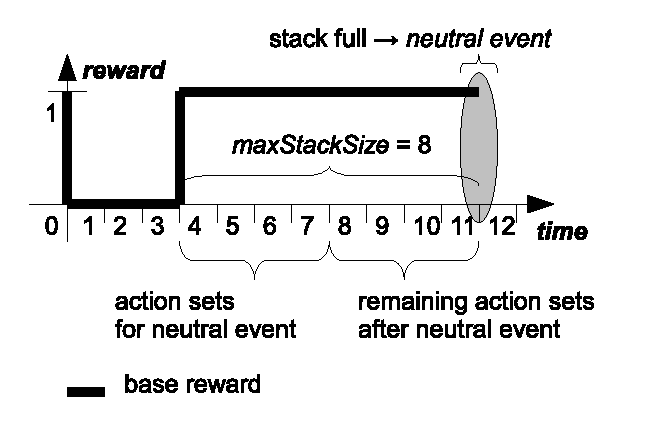
\includegraphics[scale=0.75]{neutral_event.eps}
%}
%\caption{Example of a series of base rewards that lead to neutral event (with %\emph{maxStackSize} = 8).}
%\label{figure:neutral-event}
%\end{figure}

\subsection{Reward Distribution}
\label{subsection:reward-distribution}

The standard implementation of XCS is based on the assumption that it learns within a MDP. This is expressed in the way the reward is distributed between the classifiers that contributed to reaching the goal. It requires several repetitions in order for the reward to be transferred to all classifiers that contributed to the solution.

In a dynamic scenario such repetitions are not available, the scenario is not restarted and runs continuously. This is the reason why separate measures have to be taken in order to reward previous contributing steps as well.

The approach that was used in this paper is to record not only the last action but all past actions. Such a memory mechanism does not necessarily restore the Markov property because the scenario is a NOMDP. But it does restore a direct connection of the reward between the goal and previous steps that contributed to the success (or failure).
% and an improvement in the performance is to be expected.

Thus, when (and only when) an event occurs, the reward is distributed among the entries of the action sets that were saved since the last event. With the idea in mind that recent actions probably contributed more to a positive (negative) event they are given a higher (lower) reward than to actions that were executed long time ago. 

This is done with a quadratic function which loosely resembles the transfer of the reward in the original implementation. With \(r(a)\) being the \emph{reward} for the \emph{action set} with age \(a\):
$$
r(a) = \left\{ \begin{array}{rl}
  \frac{{a}^{2}}{{\mathrm{size(\emph{action set})}}^{2}} &\mbox{ \emph{positive event}} \\
  \frac{{(1 - a)}^{2}}{{\mathrm{size(\emph{action set})}}^{2}} &\mbox{ \emph{negative event}} \\
  1 &\mbox{ \emph{neutral event}, \emph{base reward} = $1$} \\
  0 &\mbox{ \emph{neutral event}, \emph{base reward} = $0$}
       \end{array} \right.
$$

Figure~\ref{figure:saved-rewards} shows a distribution of the reward for an exemplary distribution of the base reward. For simplicity a linear distribution is displayed in the other graphics.

More sophisticated approaches are possible, this is merely the most straightforward approach. Compared to a linear distribution tests showed no significant difference. 

%\begin{figure}[ht]
%\centerline{	
%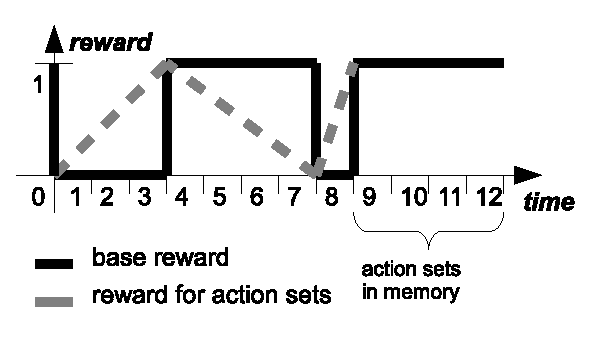
\includegraphics[scale=0.75]{saved_rewards.eps}
%}
%\caption{Schematic presentation of the reward distribution to the action sets over time after several positive and negative events}
%\label{figure:saved-rewards}
%\end{figure}
